% ---------------------------------------------------
% ----- Conclusion of the template
% ----- for Bachelor-, Master thesis and class papers
% ---------------------------------------------------
%  Created by C. Müller-Birn on 2012-08-17, CC-BY-SA 3.0.
%  Freie Universität Berlin, Institute of Computer Science, Human Centered Computing. 
%
\chapter{Implementation of Interpretability Techniques}
\label{chap:interpretability_techniques}

\section{Techniques}

Analyzing the sourced publications from \autoref{chap:literature_analysis} reveals that none of the nine potentially applicable algorithms is actually applicable to the models which were selected in the previous steps. Even if that is the case, the ideas and concepts from these techniques can be used to develop methods for this particular use case.

\subsection{Top words}

Looking at \autoref{fig:pipelinestep_gamut} shows that local instance explanations as a strategy to explain the output of an unsupervised embedding algorithm are most prevalent among all sourced publications. Factoring in the two questions from \autoref{tab:overview_viz_questions} which deal with the most prominent topics and the similarity between projects and clusters the idea arises to answer these questions by ranking the input features to the document embedding and topic extraction step for each document and cluster. According to the Gamut+ classification this would be an local instance explanation.

Assume that a document is described as a vector $c \in \mathbb{R}^k$ in the latent topic space. In order to show the most important features in the document there are two possible ways. The first option factors in how well the topic extraction projects the documents. Taking the vector in the latent space, firstly the inverse dimensionality reduction is applied in order to transform the vector into the embedding space. Both the LSA and the autodecoder approach have this opportunity, but they differ greatly in quality of this reconstruction. Since the LSA is a linear method, the back projection yields all documents on a hyperplane, while the autodecoder is able to minimize the reconstruction loss through its inherent nonlinearity. 
The second option disregards the capabilities of the topic extraction model to reconstruct a vector in the embedding space from a vector in the latent topic space. Instead for projects the embedding vector is taken directly or for cluster centers the average from all assigned projects in the embedding space is calculated as a representative. For the sake of implementational simplicity the second option was used for this thesis despite its shortcoming of disregarding the topic extraction.

Now that the document vector is in its embedding space we will make use of a special ability of the Doc2Vec model. As described in the previous section the model does not only train document vectors, but it also generates word embeddings in the same space. The revolution the Word2Vec model, as a base of the Doc2Vec model, presented was that the generated embeddings and their relations to each other encoded semantic relations. Although there is no literature on this, it is a hypothesis that this behaviour also applies to the embedding of document and word vectors into one space. This leads to the possibility of describing a document by its nearest word vectors. An exemplary analysis shows that there seems to be a valid semantic structure in the relations between tokens and between tokens and documents. As a German native speaker it is easy for me to verify that the word queries in \autoref{tab:semantic_connectivity_words} are indeed semantically well connected. The results of the document queries in \autoref{tab:semantic_connectivity_docs} on the other hand are hard to verify since most documents are very specific, scientific texts. I picked two projects and their top words which I was able to understand without relying on external information. The first three top words are indeed well connected to the topic of the corresponding project, but the last two ones seem to be off. This exemplary analysis speaks in favor of the hypothesis that there are indeed semantic connections document vectors and word vectors.

\begin{table}
	\centering
	\begin{tabular}{ p{6cm} | p{6cm} }
		"Evolution" & "Diversität" \\ \hline
		\begin{enumerate}
			\item evolutionären
			\item evolutionäre
			\item evolutionärer
			\item phylogenetische
			\item Artbildung
		\end{enumerate} & 
		\begin{enumerate}
			\item Artenzusammensetzung
			\item Biodiversität
			\item Taxa
			\item taxonomisch
			\item Lebensräumen
		\end{enumerate} \\
	\end{tabular}
	\caption{\label{tab:semantic_connectivity_words} Table showing the top five similar words for two queries by word}
\end{table}

\begin{table}
	\centering
	\begin{tabular}{ p{6cm} | p{6cm} }
		\href{https://gepris.dfg.de/gepris/projekt/387798678}{'Ambitionierte Amateure' - Europäische Filmclubs in den langen 1960er Jahren} & \href{https://gepris.dfg.de/gepris/projekt/160874660}{Netzwerke im europäischen Handel des Mittelalters} \\ \hline
		\begin{enumerate}
			\item Kulturpraxis
			\item Kulturzentren
			\item alltagsweltlich
			\item pain
			\item Ceuta
		\end{enumerate} & 
		\begin{enumerate}
			\item Opportunitätskosten
			\item Diskursteilnehmer
			\item evoluieren
			\item schloss
			\item Staphylococcen
		\end{enumerate} \\
	\end{tabular}
	\caption{\label{tab:semantic_connectivity_docs} Table showing the top five similar words for two queries by document}
\end{table}

Extracting top words for the existing TfIdf method is simpler, because every entry in the embedding vector has a one-to-one correspondence to words. Taking the biggest n entries yields n top words due to the TfIdf measure directly being a indicator for the amount of contained information and subsequently importance.

\subsection{Cluster topography }

The hypothesis on which this technique is grounded is that clusters in a high dimensional space are inherently hard to interpret, because the cluster does not exist as an explicit object. A cluster is rather an abstract concept and solely consists of the points which are connected to it via a membership assignment. Especially once the points which form a cluster get reduced into a 2D or 3D space distances and neighborhoods get distorted. Information on the position and form of the clusters is not easily obtainable anymore. One way to mitigate this is to extract artifacts in the high dimensional space and carry it over into the 2D space where the points can be visualized.

Motivated by the exploratory nature of the interaction which the non-technical experts will carry out, the quality of each point fitting into its cluster could be an interesting pointer to make potentially contrastive deductions concerning the structure of the clusters.

This technique computes an uncertainty measure for each point which describes how well it fits into its assigned cluster. A straightforward idea would be to assign each point the Euclidean distance between the point and its cluster centroid. Small distances speak in favor of the hypothesis that a point fits well into its cluster, while bigger distances speak in favor of the contrary. After the projection into 2D a topography is interpolated with the points and their Euclidean distances as fulcrums. This intendedly invokes the notion of a geographical surface since most scientists, especially at a natural history museum, work often with such kind of maps. Making sure that the peaks of this topography corresponds to points which fit very well into their clusters enlarges the metaphor and ensures that people are intuitively able to understand the visualization. 

The problem with this approach is that, firstly the Euclidean distance may not be well suited for such vector spaces, as discussed earlier, and points in different clusters cannot be compared since volume-wise larger clusters exhibit a higher distance for each point than ones which are more compact, albeit having a similar fitness in relation to the points of the same cluster. Secondly points may exhibit the same fitness and lie close together in 2D, but may be on two opposing ends of an n-dimensional sphere in the latent space. 

The second problem is harder to tackle since that is one of the inherent problems of dimensionality reductions and therefore I will present an argument for an alternative similarity measure.

The main information that this technique should convey is how well the clustering method captured the structure of the high dimensional space which can be expressed by measuring how sure the method is about the cluster assignment for each point. One measure capturing this information is the silhouette score \cite{rousseeuwSilhouettesGraphicalAid1987}. The silhouette score takes, for each sample, also the nearest, non-assigned cluster into account, computes the mean intra-cluster distance $a$ and the mean nearest-cluster distance $b$ and scores them as $\frac{(b-a)}{\max{a,b}}$. This leads to a score between -1 and 1, where a negative value denotes that the point was assigned to the wrong cluster since the nearest, not-assigned one is closer than the assigned cluster. The normalization of this score makes it possible to compare the fitness of points between clusters as well. Furthermore this proposed technique falls into the category of "Regions of error" in the Gamut+ classification - the sparsest category which only has one other paper using that strategy. 

I developed this technique in cooperation with Christoph Kinkeldey and Jesse Josua Benjamin, presented it at TrustVis19 in Porto, Portugal, as well as published it in \cite{christophkinkeldeySupportingInterpretabilityClustering2019}.

\begin{figure}[t]
	\centering
	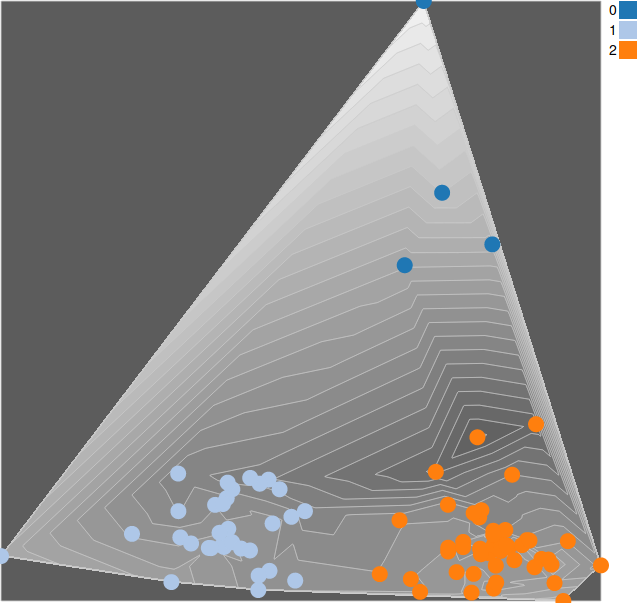
\includegraphics[width=300px]{../chapters/validation/pics/topography}
	\caption{\label{pic:topography} Screenshot showing the interpolated topography on an exemplary plot}
\end{figure}

\subsection{Linearization}

As Lipton \cite{liptonMythosModelInterpretability2016a} pointed out, a visualization is already an explainability technique in itself. Therefore we can use the vast amount of interaction design research to optimize the existing interface. 

One of the main problems of scatter graphs is overdrawing, also called clutter. This problem occurs when glyphs are close enough in a scatter plot so that they overlap each other. The higher the density of a region is, the harder it gets to perceive the total number of points and the harder it is to annotate the glyphs with additional data \cite{mayorgaSplatterplotsOvercomingOverdraw2013}. 

Normally this problem is hard to solve since the position of points in respect to each other encodes important information. Considering that in this case a high dimensional space is reduced to 2D, there are inherent reduction errors introduced into the distances between points and the absolute distances in 2D loose part of their semantic importance. Therefore it is possible to assume that instead of distances, the neighborhood of a point is more important, which leads to the possibility to map the scatter graph on a more regularized structure while preserving the neighborhood of points as well as possible. One way to do so, is to map the points in 2D onto a grid. This problem reduces to a linear assignment problem (LAP), where each point should be assigned to its nearest point in the grid while minimizing the global displacement error. A popular algorithm for that is the Jonker-Volgenant algorithm \cite{jonkerShortestAugmentingPath1987}. Jonker and Volgenant rephrase the LAP as a shortest path problem and by using augmenting paths improve the previously popular Hungarian algorithm to cubic worst-case complexity. As we will see in one of the next subsections, this technique also synergizes well with the cluster topography method, because the interpolation also get linearized and the topography gets expanded making it easier to see differences in the relief.

\begin{figure}[t]
	\centering
	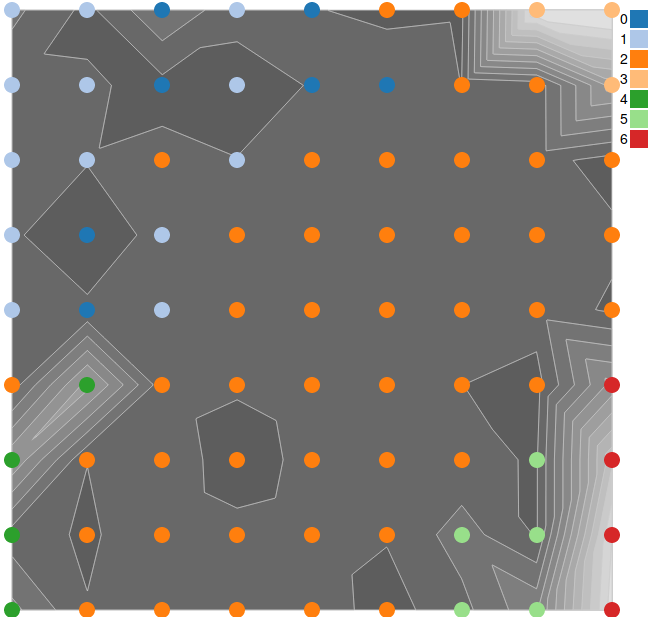
\includegraphics[width=300px]{../chapters/validation/pics/linearization}
	\caption{\label{pic:linearization} Screenshot showing the linearization on an exemplary plot}
\end{figure}

\section{Validation}

\subsection{System-Centered}

Now that there is an option to choose between two options for the embedding, topic extraction and classification step of the generic topic modeling pipeline, it is interesting to see which combination of these methods performs the best. A popular method to measure the quality of a topic modeling pipeline is the Coherence Score. Röder et al.\cite{roderExploringSpaceTopic2015a} proposed an agnostic way to evaluate topic models, unifying several contending methods at that time. Their generic pipeline consists of four steps: segmentation, probability calculation, confirmation measure and aggregation. The segmentation step consists of segmenting the dictionary, the set of all occuring words, into subsets. Then for every word a probability is calculated using a reference corpus, which is used in the subsequent step where a confirmation measure scores the word pairs concerning how often they appear together in documents or in sliding windows over documents. A last step aggregates all the agreement scores and calculates an overall coherence score for the segmentation on the supplied reference corpus. In our case the segmentation is done by supplying the top words for all clusters.  In this analysis the $c_v$ measure was chosen, because it displayed the highest correlation (0.731) with human ratings in the experiments of Röder et. al.

Plotting the coherence scores over different embedding, topic extraction and clustering models and different number of clusters reveals (\autoref{pic:tm_quality}) , surprisingly, that the combination with the best scores is an TfIdf embedding, an LSA topic extraction, followed by an Agglomerative Clustering with 10 clusters. The combination of TfIdf embeddings and an autoencoder couldn't be tested since in order to feed sparse matrices to a Keras neural network there is a considerable amount of work involved. In order to keep this thesis reasonable, this analysis was therefore excluded and is recommended for further work.

\begin{figure}[t]
	\centering
	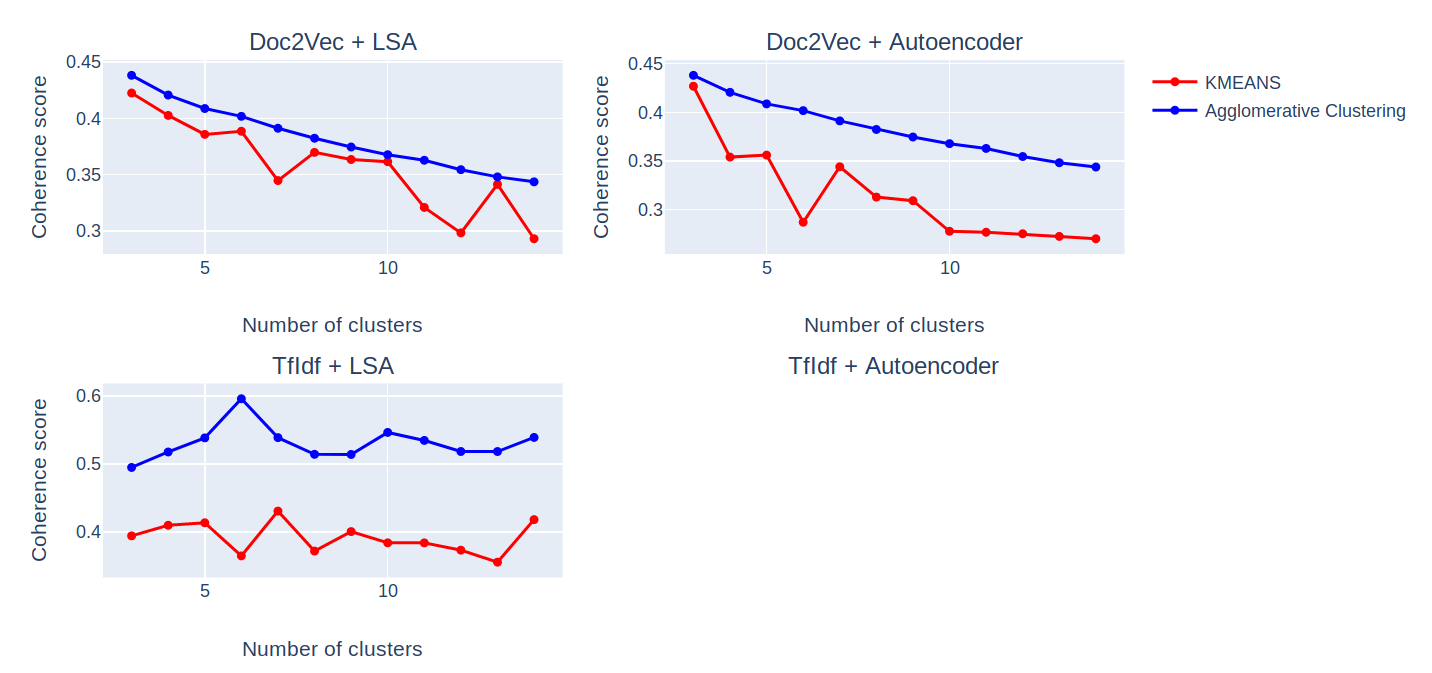
\includegraphics[width=400px]{/home/tim/HCC/IKON-backend/src/topicextraction/nlp/plots/tm_quality}
	\caption{\label{pic:tm_quality} Graph showing the quality of the topic modeling while varying the embedding, topic extraction and clustering model}
\end{figure}

Plotting this combination of models and parameters in \autoref{pic:best_coherence_plot} reveals that there is one huge cluster (cluster 0) while the other 9 clusters contain maximally five projects. A further analysis of the dominating cluster also showed that although its top words suggest projects connected to evolution and biology, there are also a number of projects which deal with geology and paleontology. Interestingly, changing the parameters of all models does not change the fact that such a huge cluster forms speaking in favor of the hypothesis that these projects indeed form a huge cluster in the high embedding space.

\begin{figure}[t]
	\centering
	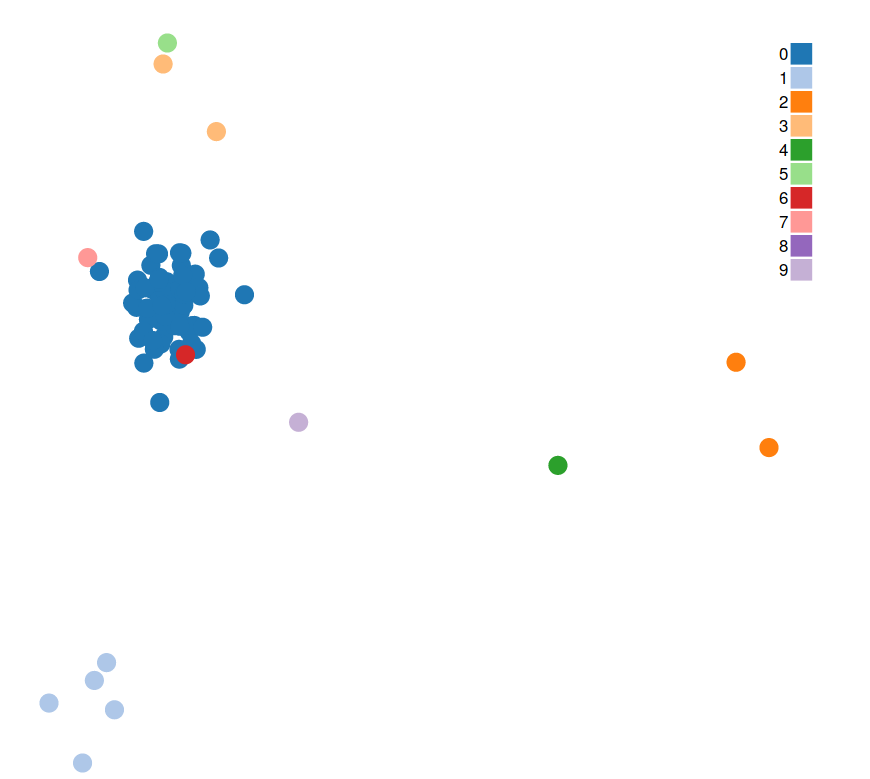
\includegraphics[width=400px]{../chapters/implementation/pics/best_coherence_plot}
	\caption{\label{pic:best_coherence_plot} Plot for the parameter and models with the best coherence score}
\end{figure}

\begin{table}
	\centering
	\begin{tabular}{c | c}
		0 & Datum, Evolution, morphologisch, Taxa, ökologisch \\ \hline
		1 & Sackflügelfledermaus, Abwanderungsverhalten, Weibchen, Männchen, Harem \\ \hline
		2 & Western, Mountains, Kaokoveld, Fauna, Escarpment \\ \hline
		3 & Tansania, biostratigraphische, palynologisch, Tendaguru, Palynologie \\ \hline
		4 & Acentropinae, Philippinen, Trichoptera, Lepidoptera, Reliktendemiten \\ \hline
		5 & SCHRANK, gesichert, Flora, Sauropoden, Gymnospermen \\ \hline
		6 & Praktik, kolonisieren, Mediziner, Gesundheitsbehörden, Malaria \\ \hline
		7 & Magmaozeans, Magmaozean, Planetare, Impaktprozess, Impaktors \\ \hline
		8 & Kurzexpedition, Basilosauridae, Pabdeh, Ablagerungen, Iran \\ \hline
		9 & Hauptexporteur, Kieselalgendiversität, Känozoikum, Silikatverwitterung, Kieselalgen \\ \hline
	\end{tabular}
	\caption{\label{tab:best_coherence_table} Table showing the top words for {\autoref{pic:best_coherence_plot}}}
\end{table}

At this point I gathered feedback from the researchers from project IKON and their answers suggested that problems may occur trying to visualize such dominating structures in scatter plots.
Therefore I turned to the second best performing combination of models which is a TfIdf embedding, an LSA topic extraction and a K-Means clustering - which is effectively the topic modeling pipeline which was existing at the beginning of the thesis. Since all the implemented explainability technique also work for this combination of methods, I sticked with it for the next validation step. 

\subsection{Human-Centered}

In order to show how the implemented explainability techniques may help a non-technical expert understanding the output generated by the pipeline, a proper user study would be needed. Since that is a task which would fill a bachelor thesis on its own, I resorted to a strategy which involves less work, but also delivers qualitative insights into the interaction between a user and the topic modeling pipeline and its visualization - the cognitive walkthrough. Performing this method involves seeing things from the perspective of a fictive user and interacting with the application in their stead.
Since the nature of this visualization supports exploratory interactions in the first place, standard approaches for cognitive walkthroughs, like they are formulated in \cite{whartonUsabilityInspectionMethods1994}, do not work well due to the necessity of coding an interaction sequence prior to the simulated interaction. Allendorf et al. \cite{allendoerferAdaptingCognitiveWalkthrough2005} adapted the well-established method of cognitive walkthroughs to this kind of use case. Their method consists of defining a persona, goals for the interaction and possible steps which can be taken in the visualization. With this setup an action is performed which seems most applicable to reach the current goal and afterwards the following four questions are answered:
\begin{enumerate}
	\item What effect was the user trying to achieve by selecting this action?
	\item How did the user know that this action was available?
	\item Did the selected action achieve the desired effect?
	\item When the action was selected, could the user determine how things were going?
\end{enumerate}

\subsubsection{Setup}
The fictive user is a postdoctoral researcher at the Museum für Naturkunde Berlin. His background is characterized by the following features:
\begin{itemize}
	\item \textbf{Education}
	Is a postdoctoral researcher of biology specializing in evolutionary theory
	
	\item \textbf{Relevant work experience}
	Currently working on a project called "Variabilität von MHC-Genen bei der Sackflügelfledermaus Saccopterix bilineata" investing the genetic variability of bats
	
	\item \textbf{Experience with user interface design and usability assessment}
	Has no prior knowledge of interface design or usability assessment
	
	\item \textbf{Operating systems and software packages used frequently}
	Microsoft Windows; Microsoft Office (Word, Excel, PowerPoint); Microsoft Outlook; Mozilla Firefox; Microsoft Media Player; LaTeX; Zotero
\end{itemize}

As described in the Introduction, there are no common meeting rooms for the scientific staff at the museum. The interface is therefore positioned on a location which has the biggest throughput in the museum - in this case the side entrance which is exclusively used by the museum's staff.
As discussed in the paragraph concerning interpretability in the Introduction, context is an essential component for interpretability. Therefore the fictive user interacts with the application in a well defined scenario:

	 One day after work, the fictive user is coming down the wide stairway of the side building he works in and sees once more the display with the visualization he passes every day on his way to and from work. This time the curiosity is stronger than the urge to go home and since he already heard that the museum financed a huge initiative to foster intra-organizational, scientific exchange, he decides to see what that application has to offer.


Looking at the questions formulated in the beginning of this thesis, we can now derive specific tasks this user may want to complete to answer the questions:
\begin{enumerate}
	\item Identify dominating research areas
	\item Find his own project
	\item Explore the projects in the same cluster
	\item Explore the projects in the vicinity of his own cluster
\end{enumerate}

The prototypical interface provides the following actions in the visualization:
\begin{enumerate}
	\item Investigate metadata for a project (title, ID and top words)
	\item Investigate top words for all clusters
	\item Change the number of clusters
	\item Switch between the linearized view and the scatter view
\end{enumerate}



\subsubsection{Cognitive Walkthrough} 

Simulating the full interaction, which is traceable in the appendix using the protocol (starting from page \pageref{ch:Appendix}),   reveals that all three implemented interpretability techniques can be used to help a fictive user understand the output of the system. The way they are used differ significantly on the other hand. 
The cluster top words were either used to quickly see what kind of topics prevail or to decide if an acceptable level of granularity was reached. If that was the case the user was able to pinpoint in which cluster the object of interest lies which reduces the search space nominally. 
The linearization was used only one time. After the user interacted with all the projects which were not hidden by clutter, they changed into the linearized view using this technique just as intended.
During the cognitive walkthrough the cluster topography was of less relevance. The user primarily used this interpretability technique to generate candidates for the next inspections via top words and not gain a global view over the clustering.

This speaks in favor of the hypothesis that interpretability techniques can be reinterpreted with another explanation strategy, as it happened with the cluster topography. This leads to the conclusion that there is not, as initially assumed, a 1:n correspondence between explanation strategies and interpretability techniques, but rather a n:n connection. Since the reinterpretation is a context-dependent step, the cognitive walkthrough, as a context-light technique, may not be the best suited for investigating the way users interpret the output of such systems. In order to research such dependencies it would be necessary to conduct a full user study in the particular environmental and mental context of the use case.

Furthermore it unveiled a number of usability issues with the visualization (\autoref{tab:usability_problems}). The first found problem is dismissable since the presented interface is not the final one which is going to go live, but the second may hinder the interaction with the visualization even in the actual prototype.

\begin{table}
	\begin{tabular}[l]{| p{.4\textwidth} | p{.6\textwidth}  |} 
		\hline
		Description & Usability Impact \\ \hline \hline
		The label for the dropdown selection between the scatter plot and the linearized view does not properly describes what it does. & 
		Uncertainty about the usage of a tool may disturb a user in the inference task, therefore a descriptive name for this selection should be chosen. \\ \hline
		There is no visual connection between views while changing the cluster or view parameters. &
		Perturbing these parameters does not change the underlying displayed corpus, but the recomputation of the full pipeline may lead, due to the random initialization of the K-Means algorithm, to dramatically different outputs. Tracking these changes is quite hard and therefore after each change the user has to orient himself in the visualization anew. Adding animated transitions could help alleviating this problems by introducing object permanence in the views. \\ \hline	
	\end{tabular}
	\caption{\label{tab:usability_problems} Table summarizing the found usability design issues} 
\end{table}

